\documentclass[a4paper, 11pt]{article}
\usepackage{graphicx}
\usepackage{multicol}
\usepackage{tabularx}
\usepackage{enumitem}
\usepackage[a4paper, margin=1.8cm]{geometry}
\usepackage{listings}
\usepackage{amssymb}
\usepackage{gvv}
\usepackage{gvv-book}
\usepackage{amsmath}
\usepackage{setspace}
\usepackage{caption}
\usepackage{tfrupee}
\usepackage{float}

\graphicspath{ {./figs/} }

\begin{document}
\begin{center}
    \huge{EC : ELECTRONICS AND COMMUNICATION ENGINEERING}\\
    \large{EE25BTECH11041 - Naman Kumar}
\end{center}

\begin{enumerate}
    \item All the four entries of the $2\times2$ matrix $P=\myvec{p_{11} & p_{12} \\ p_{21} & p_{22}}$ are nonzero, and one of its eigenvalues is zero. Which of the following statements is true?
    
    \begin{enumerate}
        \begin{multicols}{2}
            \item $p_{11}p_{22}-p_{12}p_{21}=1$
            \item $p_{11}p_{22}-p_{12}p_{21}=-1$
            \item $p_{11}p_{22}-p_{12}p_{21}=0$
            \item $p_{11}p_{22}+p_{12}p_{21}=0$
        \end{multicols}
    \end{enumerate}

    \hfill{\brak{\text{GATE EC 2008}}}

    \item The system of linear equations
    \begin{align*}
        4x+2y &= 7 \\
        2x+y &= 6
    \end{align*}
    has
    
    \begin{enumerate}
        \begin{multicols}{2}
            \item a unique solution
            \item no solution
            \item an infinite number of solutions
            \item exactly two distinct solutions
        \end{multicols}
    \end{enumerate}
    
    \hfill{\brak{\text{GATE EC 2008}}}

    \item The equation $\sin\brak{z}=10$ has
    
    \begin{enumerate}
        \begin{multicols}{2}
            \item no real or complex solution
            \item exactly two distinct complex solutions
            \item a unique solution
            \item an infinite number of complex solutions
        \end{multicols}
    \end{enumerate}
    
    \hfill{\brak{\text{GATE EC 2008}}}

    \item For real values of x, the minimum value of the function $f\brak{x}=\exp\brak{x}+\exp\brak{-x}$ is
    
    \begin{enumerate}
        \begin{multicols}{4}
            \item 2
            \item 1
            \item 0.5
            \item 0
        \end{multicols}
    \end{enumerate}
    
    \hfill{\brak{\text{GATE EC 2008}}}

    \item Which of the following functions would have only odd powers of x in its Taylor series expansion about the point $x=0$?
    
    \begin{enumerate}
        \begin{multicols}{4}
            \item $\sin\brak{x^3}$
            \item $\sin\brak{x^2}$
            \item $\cos\brak{x^3}$
            \item $\cos\brak{x^2}$
        \end{multicols}
    \end{enumerate}
    
    \hfill{\brak{\text{GATE EC 2008}}}

    \item Which of the following is a solution to the differential equation $\frac{dx\brak{t}}{dt}+3x\brak{t}=0$?
    
    \begin{enumerate}
        \begin{multicols}{2}
            \item $x\brak{t}=3e^{-t}$
            \item $x\brak{t}=2e^{-3t}$
            \item $x\brak{t}=-\frac{3}{2}t^2$
            \item $x\brak{t}=3t^2$
        \end{multicols}
    \end{enumerate}
    
    \hfill{\brak{\text{GATE EC 2008}}}
\newpage
    \item In the following graph, the number of trees \brak{P} and the number of cut-sets \brak{Q} are
    \begin{figure}[H]
        \centering
        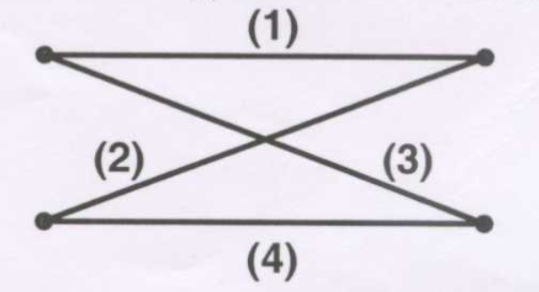
\includegraphics[width=0.4\columnwidth]{figs/q7.png}
        \caption*{}
        \label{fig:q7}
    \end{figure}
    
    \begin{enumerate}
        \begin{multicols}{4}
            \item $P=2, Q=2$
            \item $P=2, Q=6$
            \item $P=4, Q=6$
            \item $P=4, Q=10$
        \end{multicols}
    \end{enumerate}

    \hfill{\brak{\text{GATE EC 2008}}}

    \item In the following circuit, the switch S is closed at $t=0$. The rate of change of current $\frac{di}{dt}\brak{0^+}$ is given by
    \begin{figure}[H]
        \centering
        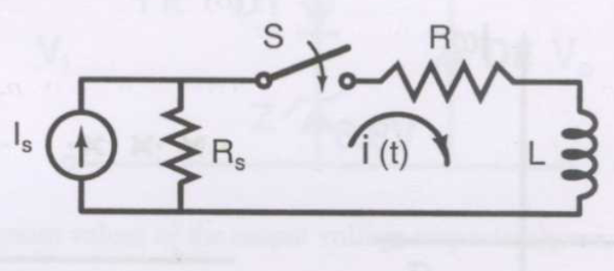
\includegraphics[width=0.6\columnwidth]{figs/q8.png}
        \caption*{}
        \label{fig:q8}
    \end{figure}
    
    \begin{enumerate}
        \begin{multicols}{2}
            \item 0
            \item $\frac{R_s I_s}{L}$
            \item $\frac{\brak{R+R_s}I_s}{L}$
            \item $\infty$
        \end{multicols}
    \end{enumerate}
    
    \hfill{\brak{\text{GATE EC 2008}}}

    \item The input and output of a continuous time system are respectively denoted by $x\brak{t}$ and $y\brak{t}$. Which of the following descriptions corresponds to a causal system?
    
    \begin{enumerate}
        \begin{multicols}{2}
            \item $y\brak{t}=x\brak{t-2}+x\brak{t+4}$
            \item $y\brak{t}=\brak{t-4}x\brak{t+1}$
            \item $y\brak{t}=\brak{t+4}x\brak{t-1}$
            \item $y\brak{t}=\brak{t+5}x\brak{t+5}$
        \end{multicols}
    \end{enumerate}
    
    \hfill{\brak{\text{GATE EC 2008}}}

    \item The impulse response $h\brak{t}$ of a linear time-invariant continuous time system is described by $h\brak{t}=\exp\brak{\alpha t}u\brak{t}+\exp\brak{\beta t}u\brak{-t}$, where $u\brak{t}$ denotes the unit step function, and $\alpha$ and $\beta$ are real constants. This system is stable if
    
    \begin{enumerate}
        \begin{multicols}{2}
            \item $\alpha$ is positive and $\beta$ is positive
            \item $\alpha$ is negative and $\beta$ is negative
            \item $\alpha$ is positive and $\beta$ is negative
            \item $\alpha$ is negative and $\beta$ is positive
        \end{multicols}
    \end{enumerate}
    
    \hfill{\brak{\text{GATE EC 2008}}}

    \item The pole-zero plot given below corresponds to a
    \begin{figure}[H]
        \centering
        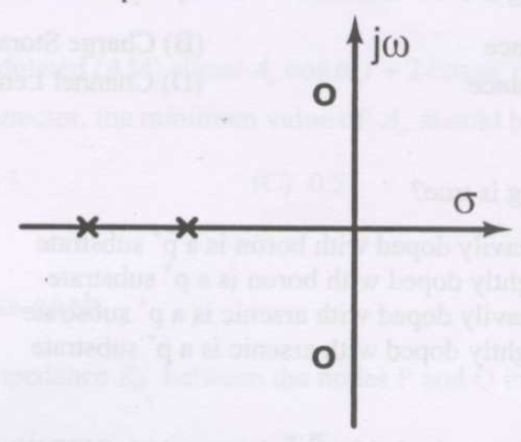
\includegraphics[width=0.4\columnwidth]{figs/q11.png}
        \caption*{}
        \label{fig:q11}
    \end{figure}
    
    \begin{enumerate}
        \begin{multicols}{2}
            \item Low pass filter
            \item High pass filter
            \item Band pass filter
            \item Notch filter
        \end{multicols}
    \end{enumerate}

    \hfill{\brak{\text{GATE EC 2008}}}

    \item Step responses of a set of three second-order underdamped systems all have the same percentage overshoot. Which of the following diagrams represents the poles of the three systems?
    \begin{enumerate}
        \item \begin{figure}[H]
        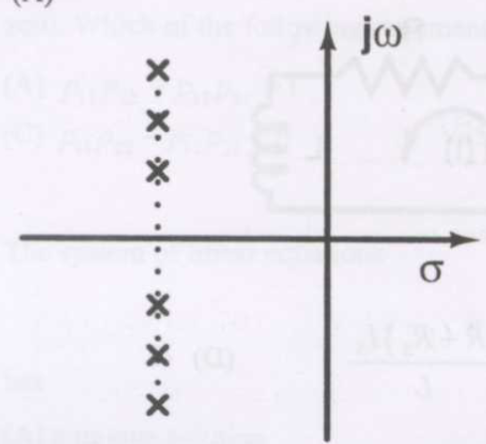
\includegraphics[width=0.2\columnwidth]{figs/q12A.png}
    \end{figure}
    \item \begin{figure}[H]
        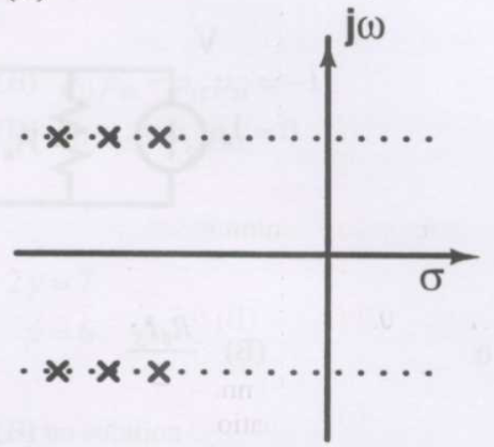
\includegraphics[width=0.2\columnwidth]{figs/q12B.png}
    \end{figure}
    \item \begin{figure}[H]
        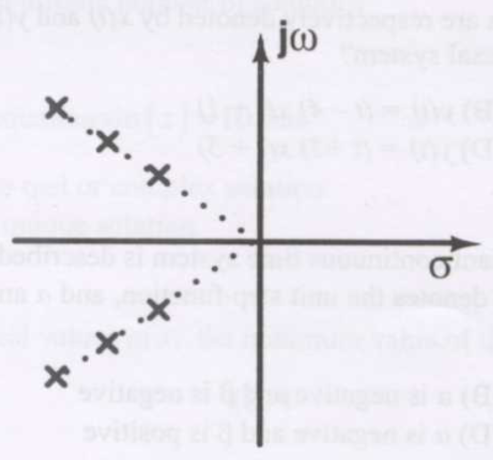
\includegraphics[width=0.2\columnwidth]{figs/q12C.png}
    \end{figure}
    \item \begin{figure}[H]
        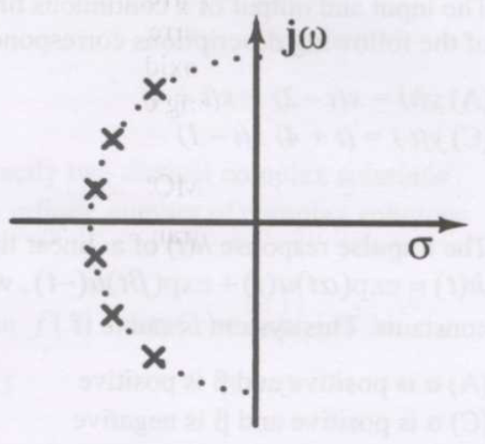
\includegraphics[width=0.2\columnwidth]{figs/q12D.png}
    \end{figure}
    \end{enumerate}

    \hfill{\brak{\text{GATE EC 2008}}}

    \item Which of the following is NOT associated with a p-n junction?
    
    \begin{enumerate}
        \begin{multicols}{2}
            \item Junction Capacitance
            \item Charge Storage Capacitance
            \item Depletion Capacitance
            \item Channel Length Modulation
        \end{multicols}
    \end{enumerate}
    
    \hfill{\brak{\text{GATE EC 2008}}}

    \item Which of the following is true?
    
    \begin{enumerate}
        \item A silicon wafer heavily doped with boron is a $p^+$ substrate
        \item A silicon wafer lightly doped with boron is a $p^+$ substrate
        \item A silicon wafer heavily doped with arsenic is a $p^+$ substrate
        \item A silicon wafer lightly doped with arsenic is a $p^+$ substrate
    \end{enumerate}

    \hfill{\brak{\text{GATE EC 2008}}}

    \item For a Hertz dipole antenna, the half power beam width \brak{HPBW} in the E-plane is
    
    \begin{enumerate}
        \begin{multicols}{4}
            \item $360\degree$
            \item $180\degree$
            \item $90\degree$
            \item $45\degree$
        \end{multicols}
    \end{enumerate}
    
    \hfill{\brak{\text{GATE EC 2008}}}

    \item For static electric and magnetic fields in an inhomogeneous source-free medium, which of the following represents the correct form of two of Maxwell's equations?
    
    \begin{enumerate}
        \begin{multicols}{4}
            \item $\nabla \cdot E = 0$ \\ $\nabla \times B = 0$
            \item $\nabla \cdot E = 0$ \\ $\nabla \cdot B = 0$
            \item $\nabla \times E = 0$ \\ $\nabla \times B = 0$
            \item $\nabla \times E = 0$ \\ $\nabla \cdot B = 0$
        \end{multicols}
    \end{enumerate}
    
    \hfill{\brak{\text{GATE EC 2008}}}
    
    \item In the following limiter circuit, an input voltage $V_i = 10 \sin 100\pi t$ is applied. Assume that the diode drop is $0.7 V$ when it is forward biased. The Zener breakdown voltage is $6.8 V$.
    \begin{figure}[H]
        \centering
        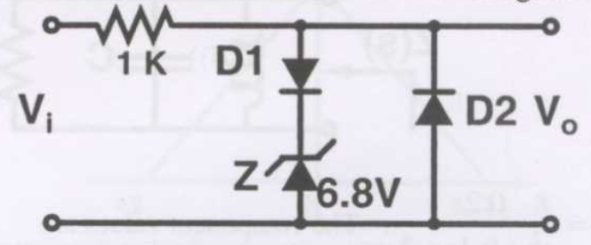
\includegraphics[width=0.5\columnwidth]{q17}
        \caption*{}
        \label{fig:q17}
    \end{figure}
    The maximum and minimum values of the output voltage respectively are
    \begin{enumerate}
        \begin{multicols}{4}
            \item $6.1 V, -0.7 V$
            \item $0.7 V, -7.5 V$
            \item $7.5 V, -0.7 V$
            \item $7.5 V, 7.5 V$
        \end{multicols}
    \end{enumerate}
    
    \hfill{\brak{\text{GATE EC 2008}}}
    
    \item A silicon wafer has $100$ nm of oxide on it and is inserted in a furnace at a temperature above $1000\degree C$ for further oxidation in dry oxygen. The oxidation rate
    \begin{enumerate}
        \item is independent of current oxide thickness and temperature
        \item is independent of current oxide thickness but depends on temperature
        \item slows down as the oxide grows
        \item is zero as the existing oxide prevents further oxidation
    \end{enumerate}
    
    \hfill{\brak{\text{GATE EC 2008}}}

    \item The drain current of a MOSFET in saturation is given by $I_D = K\brak{V_{GS}-V_T}^2$ where K is a constant. The magnitude of the transconductance $g_m$ is
    
    \begin{enumerate}
        \begin{multicols}{2}
            \item $\frac{K\brak{V_{GS}-V_T}^2}{V_{DS}}$
            \item $2K\brak{V_{GS}-V_T}$
            \item $\frac{I_d}{V_{GS}-V_{DS}}$
            \item $\frac{K\brak{V_{GS}-V_T}^2}{V_{GS}}$
        \end{multicols}
    \end{enumerate}

    \hfill{\brak{\text{GATE EC 2008}}}

    \item Consider the amplitude modulated \brak{AM} signal $A_c \cos\omega_c t + 2 \cos\omega_m t \cos\omega_c t$. For demodulating the signal using envelope detector, the minimum value of $A_c$ should be
    
    \begin{enumerate}
        \begin{multicols}{4}
            \item $2$
            \item $1$
            \item $0.5$
            \item $0$
        \end{multicols}
    \end{enumerate}
    
    \hfill{\brak{\text{GATE EC 2008}}}

    \item The Thevenin equivalent impedance $Z_{th}$ between the nodes P and Q in the following circuit is
    \begin{figure}[H]
        \centering
        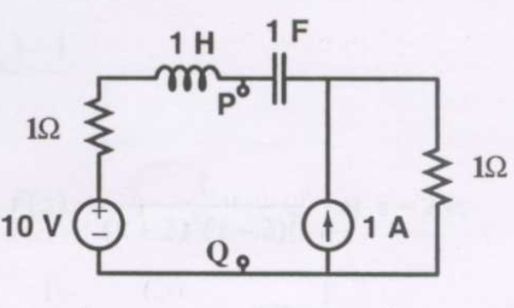
\includegraphics[width=0.6\columnwidth]{figs/q21.png}
        \caption*{}
        \label{fig:q21}
    \end{figure}
    \begin{enumerate}
        \item 1
        \item $1+s+\frac{1}{s}$
        \item $2+s+\frac{1}{s}$
        \item $\frac{s^2+s+1}{s^2+2s+1}$
    \end{enumerate}
    
    \hfill{\brak{\text{GATE EC 2008}}}

    \item The driving point impedance of the following network
    \begin{figure}[H]
        \centering
        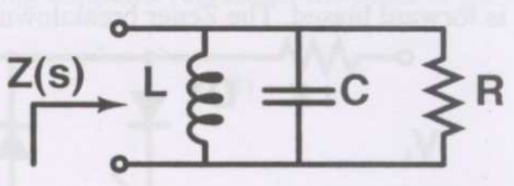
\includegraphics[width=0.3\columnwidth]{figs/q22.png}
        \caption*{}
        \label{fig:q22}
    \end{figure}
    is given by $Z\brak{s} = \frac{0.2s}{s^2+0.1s+2}$. The component values are
    \begin{enumerate}
        \begin{multicols}{2}
            \item $L=5H, R=0.5\ohm, C=0.1F$
            \item $L=0.1H, R=0.5\ohm, C=5F$
            \item $L=5H, R=2\ohm, C=0.1F$
            \item $L=0.1H, R=2\ohm, C=5F$
        \end{multicols}
    \end{enumerate}
    
    \hfill{\brak{\text{GATE EC 2008}}}

    \item The circuit shown in the figure is used to charge the capacitor C alternately from two current sources as indicated. The switches S1 and S2 are mechanically coupled and connected as follows:\\For $2nT \le t < \brak{2n+1}T$, \quad \brak{n=0,1,2,...}   S1 to P1 and S2 to P2.\\For $\brak{2n+1}T \le t < \brak{2n+2}T$, \quad \brak{n=0,1,2,...}   S1 to Q1 and S2 to Q2.
    \begin{figure}[H]
        \centering
        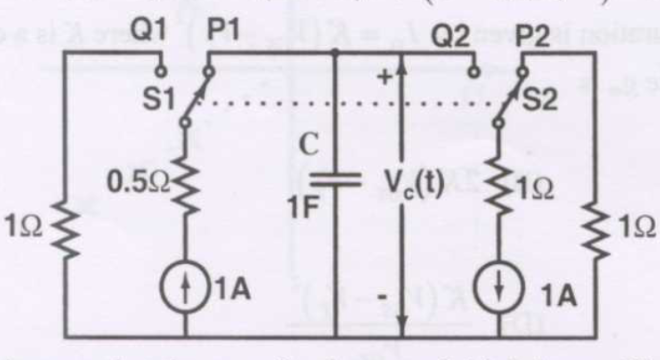
\includegraphics[width=0.7\columnwidth]{figs/q23.png}
    \end{figure}
    Assume that the capacitor has zero initial charge. Given that $u\brak{t}$ is a unit step function, the voltage $V_c\brak{t}$ across the capacitor is given by
    \begin{enumerate}
        \item $\sum_{n=0}^{\infty}\brak{-1}^n t u\brak{t-nT}$
        \item $u\brak{t} + 2 \sum_{n=1}^{\infty}\brak{-1}^n u\brak{t-nT}$
        \item $t u\brak{t} + 2 \sum_{n=1}^{\infty}\brak{-1}^n \brak{t-nT} u\brak{t-nT}$
        \item $\sum_{n=0}^{\infty} [0.5 - e^{-\brak{t-2nT}} + 0.5e^{-\brak{t-2nT-T}}]$
    \end{enumerate}
    
    \hfill{\brak{\text{GATE EC 2008}}}

    \item The probability density function \brak{PDF} of a random variable X is as shown below.
    \begin{figure}[H]
        \centering
        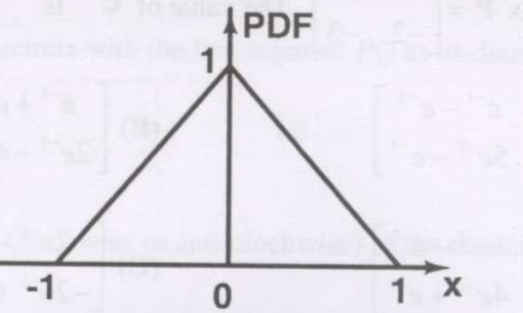
\includegraphics[width=0.4\columnwidth]{figs/q24.png}
    \end{figure}
    The corresponding cumulative distribution function \brak{CDF} has the form
    \begin{figure}[H]
        \centering
        \begin{minipage}{0.45\textwidth}
            \centering
            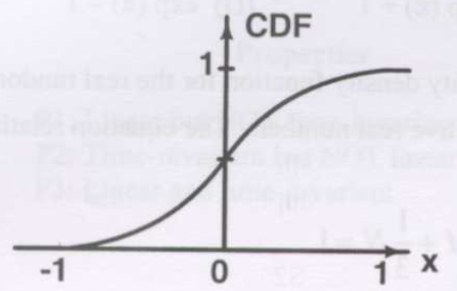
\includegraphics[width=0.8\columnwidth]{figs/q24A.png}
            \centerline{\brak{A}}
        \end{minipage}
        \hfill
        \begin{minipage}{0.45\textwidth}
            \centering
            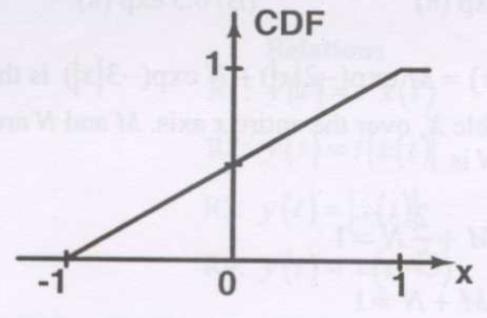
\includegraphics[width=0.8\columnwidth]{figs/q24b.png}
            \centerline{\brak{B}}
        \end{minipage}
        \vfill
        \begin{minipage}{0.45\textwidth}
            \centering
            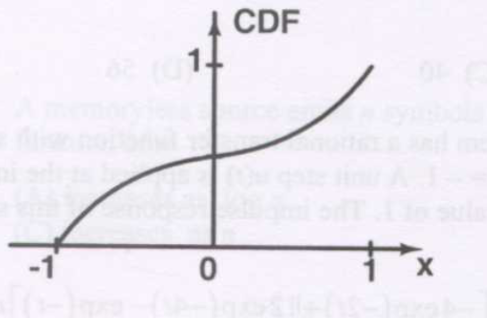
\includegraphics[width=0.8\columnwidth]{figs/q24C.png}
            \centerline{\brak{C}}
        \end{minipage}
        \hfill
        \begin{minipage}{0.45\textwidth}
            \centering
            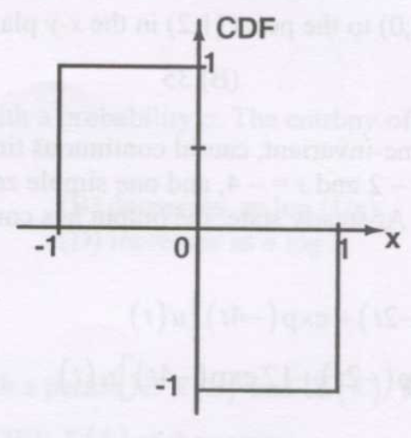
\includegraphics[width=0.8\columnwidth]{figs/q24D.png}
            \centerline{\brak{D}}
        \end{minipage}
        \caption*{}
        \label{fig:q24_options}
    \end{figure}

    \hfill{\brak{\text{GATE EC 2008}}}

    \item The recursion relation to solve $x=e^{-x}$ using Newton-Raphson method is
    \begin{enumerate}
        \begin{multicols}{2}
            \item $x_{n+1}=e^{-x_n}$
            \item $x_{n+1}=x_n-e^{-x_n}$
            \item $x_{n+1}=\brak{1+x_n}\frac{e^{-x_n}}{1+e^{-x_n}}$
            \item $x_{n+1}=\frac{x_n^2-e^{-x_n}\brak{1+x_n}-1}{x_n-e^{-x_n}}$
        \end{multicols}
    \end{enumerate}

    \hfill{\brak{\text{GATE EC 2008}}}

    \item The residue of the function $f\brak{z} = \frac{1}{\brak{z+2}^2\brak{z-2}^2}$ at $z=2$ is
    \begin{enumerate}
        \begin{multicols}{4}
            \item $-\frac{1}{32}$
            \item $-\frac{1}{16}$
            \item $\frac{1}{16}$
            \item $\frac{1}{32}$
        \end{multicols}
    \end{enumerate}
    
    \hfill{\brak{\text{GATE EC 2008}}}

    \item Consider the matrix $P=\myvec{0 & 1 \\ -2 & -3}$. The value of $e^P$ is
    \begin{enumerate}
        \item $\myvec{2e^{-2}-3e^{-1} & e^{-1}-e^{-2} \\ 2e^{-2}-2e^{-1} & 5e^{-2}-e^{-1}}$
        \item $\myvec{e^{-1}+e^{-2} & 2e^{-2}-e^{-1} \\ 2e^{-1}-4e^{-2} & 3e^{-1}+2e^{-2}}$
        \item $\myvec{5e^{-2}-e^{-1} & 3e^{-1}-e^{-2} \\ 2e^{-2}-6e^{-1} & 4e^{-2}+e^{-1}}$
        \item $\myvec{2e^{-1}-e^{-2} & e^{-1}-e^{-2} \\ -2e^{-1}+2e^{-2} & -e^{-1}+2e^{-2}}$
    \end{enumerate}

    \hfill{\brak{\text{GATE EC 2008}}}

    \item In the Taylor series expansion of $\exp\brak{x}+\sin\brak{x}$ about the point $x=\pi$, the coefficient of $\brak{x-\pi}^2$ is
    \begin{enumerate}
        \begin{multicols}{4}
            \item $\exp\brak{\pi}$
            \item $0.5 \exp\brak{\pi}$
            \item $\exp\brak{\pi}+1$
            \item $\exp\brak{\pi}-1$
        \end{multicols}
    \end{enumerate}
    
    \hfill{\brak{\text{GATE EC 2008}}}

    \item $P_x\brak{x}=M\exp\brak{-2|x|}+N\exp\brak{-3|x|}$ is the probability density function for the real random variable X, over the entire x axis. M and N are both positive real numbers. The equation relating M and N is
    
    \begin{enumerate}
        \begin{multicols}{2}
            \item $M + \frac{2}{3}N = 1$
            \item $2M+\frac{1}{3}N=1$
            \item $M+N=1$
            \item $M+N=3$
        \end{multicols}
    \end{enumerate}
    
    \hfill{\brak{\text{GATE EC 2008}}}
    
    \item The value of the integral of the function $g\brak{x,y}=4x^3+10y^4$ along the straight line segment from the point \brak{0,0} to the point \brak{1,2} in the x-y plane is
    
    \begin{enumerate}
        \begin{multicols}{4}
            \item 33
            \item 35
            \item 40
            \item 56
        \end{multicols}
    \end{enumerate}
    
    \hfill{\brak{\text{GATE EC 2008}}}
    
    \item A linear, time-invariant, causal continuous time system has a rational transfer function with simple poles at $s=-2$ and $s=-4$, and one simple zero at $s=-1$. A unit step $u\brak{t}$ is applied at the input of the system. At steady state, the output has constant value of 1. The impulse response of this system is
    
    \begin{enumerate}
    \begin{multicols}{2}
        \item $[\exp\brak{-2t}+\exp\brak{-4t}]u\brak{t}$
        \item $[-4\exp\brak{-2t}+12\exp\brak{-4t}-\exp\brak{-t}]u\brak{t}$
        \item $[-4\exp\brak{-2t}+12\exp\brak{-4t}]u\brak{t}$
        \item $[-0.5\exp\brak{-2t}+1.5\exp\brak{-4t}]u\brak{t}$
    \end{multicols}
    \end{enumerate}
    
    \hfill{\brak{\text{GATE EC 2008}}}
    
    \item The signal $x\brak{t}$ is described by
    \[ x\brak{t} = \begin{cases} 1 & \text{for } -1 \le t \le +1 \\ 0 & \text{otherwise} \end{cases} \]
    Two of the angular frequencies at which its Fourier transform becomes zero are
    
    \begin{enumerate}
        \begin{multicols}{2}
            \item $\pi, 2\pi$
            \item $0.5\pi, 1.5\pi$
            \item $0, \pi$
            \item $2\pi, 2.5\pi$
        \end{multicols}
    \end{enumerate}
    
    \hfill{\brak{\text{GATE EC 2008}}}
    
    \item A discrete time linear shift-invariant system has an impulse response $h[n]$ with $h[0]=1, h[1]=-1, h[2]=2,$ and zero otherwise. The system is given an input sequence $x[n]$ with $x[0]=x[2]=1,$ and zero otherwise. The number of nonzero samples in the output sequence $y[n]$, and the value of y[2] are, respectively
    
    \begin{enumerate}
        \begin{multicols}{2}
            \item 5, 2
            \item 6, 2
            \item 6, 1
            \item 5, 3
        \end{multicols}
    \end{enumerate}
    
    \hfill{\brak{\text{GATE EC 2008}}}

    \item Consider points P and Q in the x-y plane, with $P=\brak{1,0}$ and $Q=\brak{0,1}$. The line integral $2\int_{P}^{Q}\brak{xdx+ydy}$ along the semicircle with the line segment PQ as its diameter
    \begin{enumerate}
            \item is -1
            \item is 0
            \item is 1\textbf{}
            \item depends on the direction \brak{clockwise or anti-clockwise} of the semicircle
    \end{enumerate}
    
    \hfill{\brak{\text{GATE EC 2008}}}

    \item Let $x\brak{t}$ be the input and $y\brak{t}$ be the output of a continuous time system. Match the system properties P1, P2 and P3 with system relations R1, R2, R3, R4.\\
    \begin{tabular}{ll}
        Properties & Relations\\
        \textbf{P1}: Linear but NOT time-invariant & \textbf{R1}: $y\brak{t}=t^2x\brak{t}$ \\
        \textbf{P2}: Time-invariant but NOT linear & \textbf{R2}: $y\brak{t}=t|x\brak{t}|$ \\
        \textbf{P3}: Linear and time-invariant & \textbf{R3}: $y\brak{t}=|x\brak{t}|$\\
         & \textbf{R4}: $y\brak{t}=x\brak{t-5}$
    \end{tabular}

    
    \begin{enumerate}
        \begin{multicols}{2}
            \item \brak{P1, R1}, \brak{P2, R3}, \brak{P3, R4}
            \item \brak{P1, R2}, \brak{P2, R3}, \brak{P3, R4}
            \item \brak{P1, R3}, \brak{P2, R1}, \brak{P3, R2}
            \item \brak{P1, R1}, \brak{P2, R2}, \brak{P3, R3}
        \end{multicols}
    \end{enumerate}
    
    \hfill{\brak{\text{GATE EC 2008}}}
    
    \item A memoryless source emits n symbols each with a probability p. The entropy of the source as a function of n
    \begin{enumerate}
        \begin{multicols}{2}
            \item increases as $\log n$
            \item decreases as $\log\brak{1/n}$
            \item increases as n
            \item increases as n $\log n$
        \end{multicols}
    \end{enumerate}

    \hfill{\brak{\text{GATE EC 2008}}}

    \item $\{x\brak{n}\}$ is a real-valued periodic sequence with a period N. $x\brak{n}$ and $X\brak{k}$ form N-point Discrete Fourier Transform \brak{DFT} pairs. The DFT $Y\brak{k}$ of the sequence\\ $y\brak{n} = \frac{1}{N}\sum_{r=0}^{N-1}x\brak{r}x\brak{n+r}$ is
    \begin{enumerate}
        \begin{multicols}{2}
            \item $|X\brak{k}|^2$
            \item $\frac{1}{N}\sum_{r=0}^{N-1}X\brak{r}X^*\brak{k+r}$
            \item $\frac{1}{N}\sum_{r=0}^{N-1}X\brak{r}X\brak{k+r}$
            \item 0
        \end{multicols}
    \end{enumerate}
    
    \hfill{\brak{\text{GATE EC 2008}}}
    
    \newpage
    \item Group I lists a set of four transfer functions. Group II gives a list of possible step responses y\brak{t}. Match the step responses with the corresponding transfer functions.
    \textbf{Group I}
    \begin{description}
    \begin{multicols}{4}
        \item[P =] $\frac{25}{s^2+25}$
        \item[Q =] $\frac{36}{s^2+20s+36}$
        \item[R =] $\frac{36}{s^2+12s+36}$
        \item[S =] $\frac{49}{s^2+7s+49}$
    \end{multicols}
    \end{description}
    \textbf{Group II}
    \begin{figure}[H]
        \centering
        \begin{minipage}{0.45\textwidth}
            \centering
            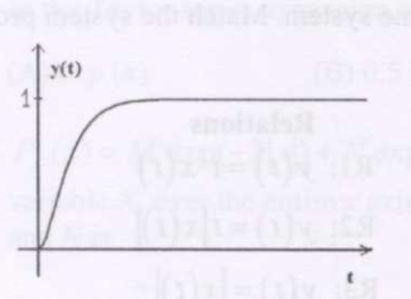
\includegraphics[width=0.9\columnwidth]{figs/q38A.png}
            \centerline{1.}
        \end{minipage}
        \hfill
        \begin{minipage}{0.45\textwidth}
            \centering
            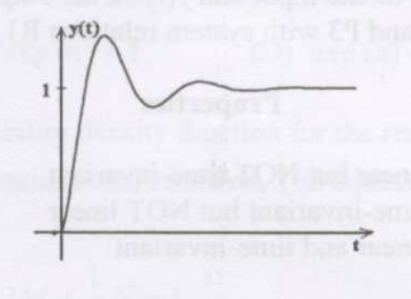
\includegraphics[width=0.9\columnwidth]{figs/q38B.png}
            \centerline{2.}
        \end{minipage}
        \vfill
        \begin{minipage}{0.45\textwidth}
            \centering
            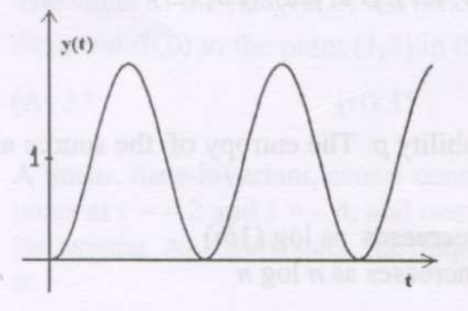
\includegraphics[width=0.9\columnwidth]{figs/q38C.png}
            \centerline{3.}
        \end{minipage}
        \hfill
        \begin{minipage}{0.45\textwidth}
            \centering
            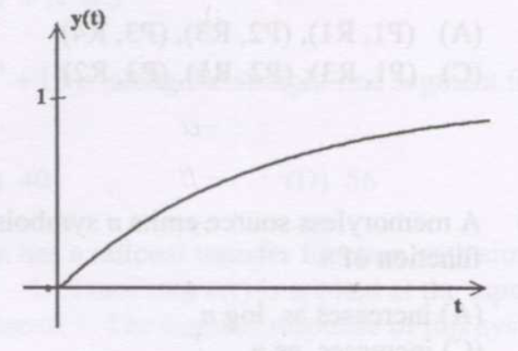
\includegraphics[width=0.9\columnwidth]{figs/q38D.png}
            \centerline{4.}
        \end{minipage}
        \caption*{}
        \label{fig:q38_options}
    \end{figure}
    
    \begin{enumerate}
        \begin{multicols}{2}
            \item P-3, Q-1, R-4, S-2
            \item P-3, Q-2, R-4, S-1
            \item P-2, Q-1, R-4, S-3
            \item P-3, Q-4, R-1, S-2
        \end{multicols}
    \end{enumerate}

    \hfill{\brak{\text{GATE EC 2008}}}
    
    \item A certain system has transfer function $G\brak{s} = \frac{s+8}{s^2+\alpha s - 4}$ where $\alpha$ is a parameter. Consider the standard negative unity feedback configuration as shown below.
    \begin{figure}[H]
        \centering
        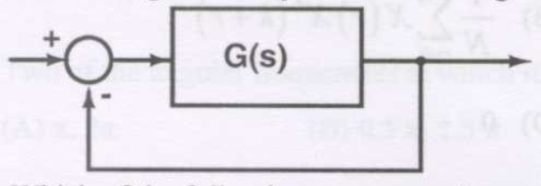
\includegraphics[width=0.5\columnwidth]{figs/q39.png}
        \caption*{}
        \label{fig:q39}
    \end{figure}
    Which of the following statements is true?
    \begin{enumerate}
        \item The closed loop system is never stable for any value of $\alpha$.
        \item For some positive values of $\alpha$, the closed loop system is stable, but not for all positive values.
        \item For all positive values of $\alpha$, the closed loop system is stable.
        \item The closed loop system is stable for all values of $\alpha$, both positive and negative.
    \end{enumerate}
    
    \hfill{\brak{\text{GATE EC 2008}}}
    
    \item A signal flow graph of a system is given below.
    \begin{figure}[H]
        \centering
        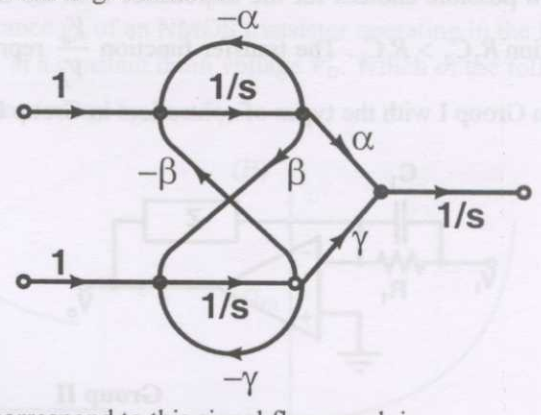
\includegraphics[width=0.7\columnwidth]{q40}
        \caption*{}
        \label{fig:q40}
    \end{figure}
    The set of equations that correspond to this signal flow graph is
    \begin{enumerate}
        \item $\frac{d}{dt}\myvec{x_1 \\ x_2 \\ x_3} = \myvec{\beta & -\gamma & 0 \\ \gamma & \alpha & 0 \\ -\alpha & -\beta & 0}\myvec{x_1 \\ x_2 \\ x_3} + \myvec{1 & 0 \\ 0 & 0 \\ 0 & 1}\myvec{u_1 \\ u_2}$
        \item $\frac{d}{dt}\myvec{x_1 \\ x_2 \\ x_3} = \myvec{0 & \alpha & \gamma \\ 0 & -\alpha & -\gamma \\ 0 & \beta & -\beta}\myvec{x_1 \\ x_2 \\ x_3} + \myvec{0 & 0 \\ 0 & 1 \\ 1 & 0}\myvec{u_1 \\ u_2}$
        \item $\frac{d}{dt}\myvec{x_1 \\ x_2 \\ x_3} = \myvec{-\alpha & \beta & 0 \\ -\beta & -\gamma & 0 \\ \alpha & \gamma & 0}\myvec{x_1 \\ x_2 \\ x_3} + \myvec{1 & 0 \\ 0 & 1 \\ 0 & 0}\myvec{u_1 \\ u_2}$
        \item $\frac{d}{dt}\myvec{x_1 \\ x_2 \\ x_3} = \myvec{-\gamma & 0 & \beta \\ \gamma & 0 & \alpha \\ -\beta & 0 & -\alpha}\myvec{x_1 \\ x_2 \\ x_3} + \myvec{0 & 1 \\ 0 & 0 \\ 1 & 0}\myvec{u_1 \\ u_2}$
    \end{enumerate}
    
    \hfill{\brak{\text{GATE EC 2008}}}
    
    \item The number of open right half plane poles of $G\brak{s} = \frac{10}{s^5+2s^4+3s^3+6s^2+5s+3}$ is
    \begin{enumerate}
        \begin{multicols}{4}
            \item 0
            \item 1
            \item 2
            \item 3
        \end{multicols}
    \end{enumerate}
    
    \hfill{\brak{\text{GATE EC 2008}}}
    
    \item The magnitude of frequency response of an underdamped second order system is 5 at 0 rad/sec and peaks to $\frac{10}{\sqrt{3}}$ at $5\sqrt{2}$ rad/sec. The transfer function of the system is
    \begin{enumerate}
        \begin{multicols}{2}
            \item $\frac{500}{s^2+10s+100}$
            \item $\frac{375}{s^2+5s+75}$
            \item $\frac{720}{s^2+12s+144}$
            \item $\frac{1125}{s^2+25s+225}$
        \end{multicols}
    \end{enumerate}
    
    \hfill{\brak{\text{GATE EC 2008}}}

    \item Group I gives two possible choices for the impedance Z in the diagram. The circuit elements in Z satisfy the condition $R_2C_2 > R_1C_1$. The transfer function $\frac{V_o}{V_i}$ represents a kind of controller. Match the impedances in Group I with the types of controllers in Group II.
    \begin{figure}[H]
        \centering
        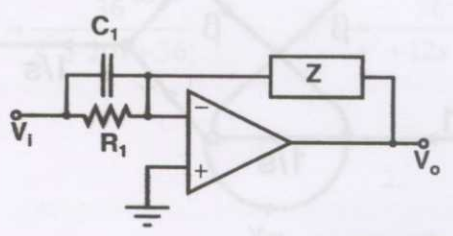
\includegraphics[width=0.6\columnwidth]{figs/q43.png}
        \caption*{}
        \label{fig:q43}
    \end{figure}
    
    \begin{minipage}{0.45\textwidth}
        \textbf{Group I}
        \begin{description}
            \item[Q.] 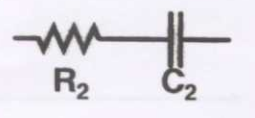
\includegraphics[width=0.4\columnwidth]{figs/q43Q.png}
            \item[R.] 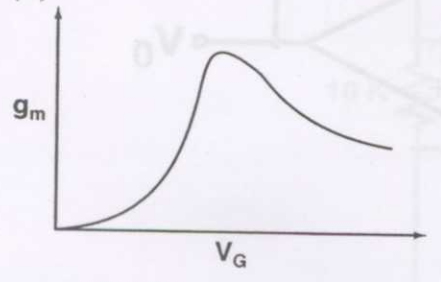
\includegraphics[width=0.4\columnwidth]{figs/q45A.png}
        \end{description}
    \end{minipage}
    \begin{minipage}{0.45\textwidth}
        \textbf{Group II}
        \begin{enumerate}
            \item PID controller
            \item Lead compensator
            \item Lag compensator
        \end{enumerate}
    \end{minipage}

    \begin{enumerate}
        \begin{multicols}{2}
            \item Q-1, R-2
            \item Q-1, R-3
            \item Q-2, R-3
            \item Q-3, R-2
        \end{multicols}
    \end{enumerate}

    \hfill{\brak{\text{GATE EC 2008}}}
    \newpage
    \item For the circuit shown in the following figure, transistors M1 and M2 are identical NMOS transistors. Assume that M2 is in saturation and the output is unloaded.
    \begin{figure}[H]
        \centering
        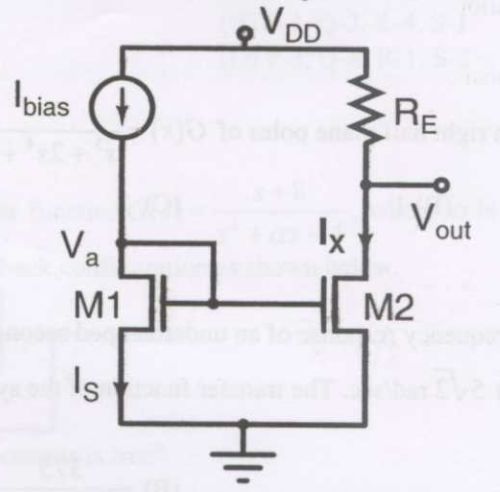
\includegraphics[width=0.5\columnwidth]{q44}
        \caption*{}
        \label{fig:q44}
    \end{figure}
    The current $I_x$ is related to $I_{bias}$ as
    \begin{enumerate}
        \begin{multicols}{2}
            \item $I_x = I_{bias} + I_s$
            \item $I_x = I_{bias}$
            \item $I_x = I_{bias} - I_s$
            \item $I_x = I_{bias} - \brak{V_{DD}-\frac{V_{out}}{R_E}}$
        \end{multicols}
    \end{enumerate}
    
    \hfill{\brak{\text{GATE EC 2008}}}

    \item The measured transconductance $g_m$ of an NMOS transistor operating in the linear region is plotted against the gate voltage $V_G$ at a constant drain voltage $V_D$. Which of the following figures represents the expected dependence of $g_m$ on $V_G$?
    \begin{figure}[H]
        \centering
        \begin{minipage}{0.45\textwidth}
            \centering
            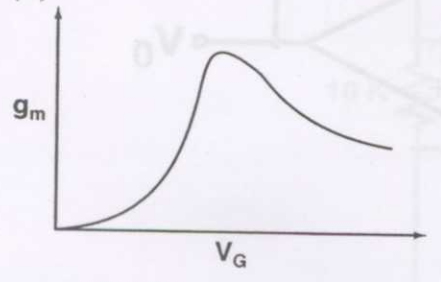
\includegraphics[width=0.8\columnwidth]{figs/q45A.png}
            \centerline{\brak{A}}
        \end{minipage}
        \hfill
        \begin{minipage}{0.45\textwidth}
            \centering
            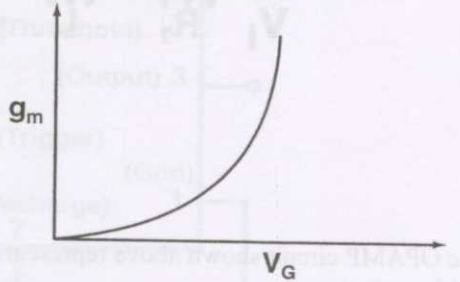
\includegraphics[width=0.8\columnwidth]{figs/q45B.png}
            \centerline{\brak{B}}
        \end{minipage}
        \vfill
        \begin{minipage}{0.45\textwidth}
            \centering
            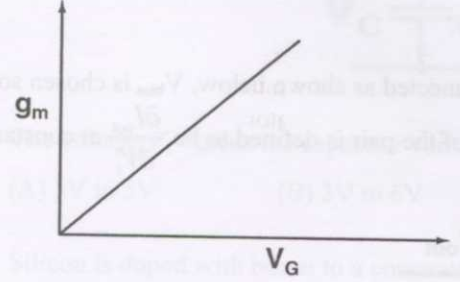
\includegraphics[width=0.8\columnwidth]{figs/q45C.png}
            \centerline{\brak{C}}
        \end{minipage}
        \hfill
        \begin{minipage}{0.45\textwidth}
            \centering
            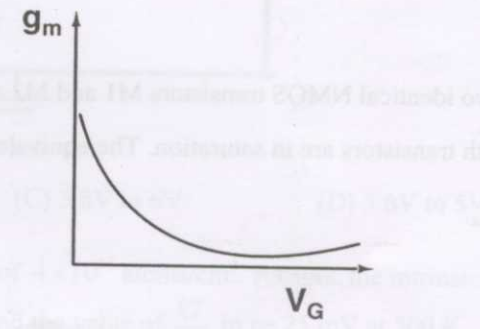
\includegraphics[width=0.8\columnwidth]{figs/q45D.png}
            \centerline{\brak{D}}
        \end{minipage}
        \caption*{}
        \label{fig:q45_options}
    \end{figure}

    \hfill{\brak{\text{GATE EC 2008}}}
    
    \item Consider the following circuit using an ideal OPAMP. The I-V characteristics of the diode is described by the relation $I = I_0\brak{e^{\frac{V}{V_T}}-1}$ where $V_T=25mV$, $I_0=1\mu A$ and V is the voltage across the diode \brak{taken as positive for forward bias}.
    \begin{figure}[H]
        \centering
        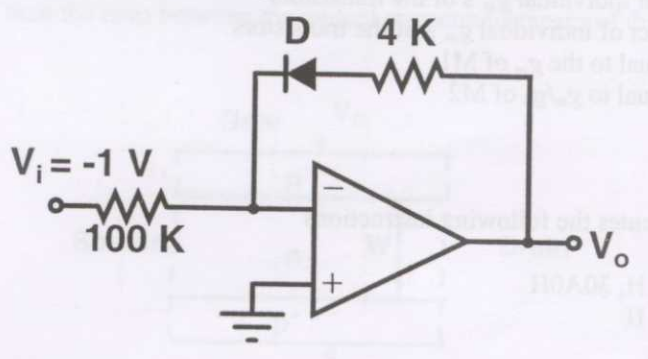
\includegraphics[width=0.6\columnwidth]{q46}
        \caption*{}
        \label{fig:q46}
    \end{figure}
    For an input voltage $V_i = -1V$, the output voltage $V_o$ is
    \begin{enumerate}
        \begin{multicols}{4}
            \item 0 V
            \item 0.1 V
            \item 0.7 V
            \item 1.1 V
        \end{multicols}
    \end{enumerate}
    
    \hfill{\brak{\text{GATE EC 2008}}}
    
    \item The OPAMP circuit shown above represents a
    \begin{figure}[H]
        \centering
        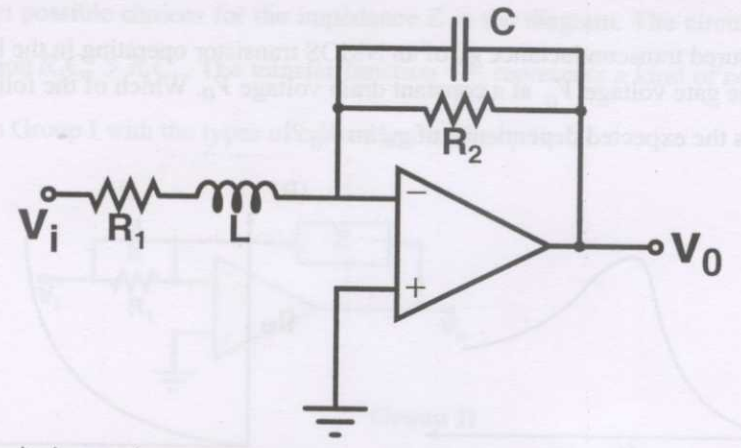
\includegraphics[width=0.7\columnwidth]{q47}
        \caption*{}
        \label{fig:q47}
    \end{figure}
    \begin{enumerate}
        \begin{multicols}{4}
            \item high pass filter
            \item low pass filter
            \item band pass filter
            \item band reject filter
        \end{multicols}
    \end{enumerate}

    \hfill{\brak{\text{GATE EC 2008}}}

    \item Two identical NMOS transistors M1 and M2 are connected as shown below. $V_{bias}$ is chosen so that both transistors are in saturation. The equivalent $g_m$ of the pair is defined to be $\frac{\partial I_{out}}{\partial V_i}$ at constant $V_{out}$.
    \begin{figure}[H]
        \centering
        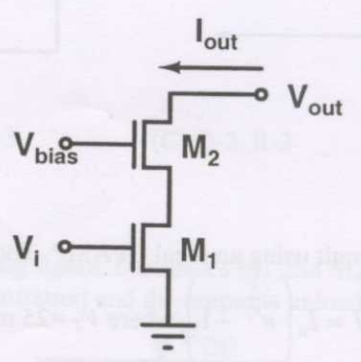
\includegraphics[width=0.3\columnwidth]{q48}
        \caption*{}
        \label{fig:q48}
    \end{figure}
    The equivalent $g_m$ of the pair is
    \begin{enumerate}
        \item the sum of individual $g_m$ of the transistors
        \item the product of individual $g_m$ of the transistors
        \item nearly equal to the $g_m$ of M1
        \item nearly equal to $g_m/g_o$ of M2
    \end{enumerate}

    \hfill{\brak{\text{GATE EC 2008}}}
    
    \item An 8085 executes the following instructions
    \begin{lstlisting}
    2710 LXI H, 30A0H
    2713 DAD H
    2714 PCHL
    \end{lstlisting}
    All addresses and constants are in Hex. Let PC be the contents of the program counter and HL be the contents of the HL register pair just after executing PCHL. Which of the following statements is correct
    
    \begin{enumerate}
        \begin{multicols}{2}
            \item $PC = 2715H, HL=30A0H$
            \item $PC = 30A0H, HL=2715H$
            \item $PC = 6140H, HL=6140H$
            \item $PC = 6140H, HL=2715H$
        \end{multicols}
    \end{enumerate}
    
    \hfill{\brak{\text{GATE EC 2008}}}
    
    \item An astable multivibrator circuit using IC 555 timer is shown below. Assume that the circuit is oscillating steadily.
    \begin{figure}[H]
        \centering
        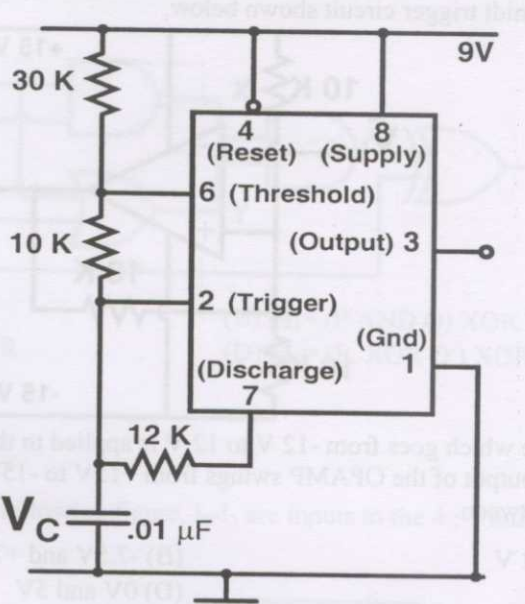
\includegraphics[width=0.5\columnwidth]{q50}
        \caption*{}
        \label{fig:q50}
    \end{figure}
    The voltage $V_C$ across the capacitor varies between
    \begin{enumerate}
        \begin{multicols}{2}
            \item 3V to 5V
            \item 3V to 6V
            \item 3.6V to 6V
            \item 3.6V to 5V
        \end{multicols}
    \end{enumerate}
    
    \hfill{\brak{\text{GATE EC 2008}}}
    
    \item Silicon is doped with boron to a concentration of $4 \times 10^{17} atoms/cm^3$. Assume the intrinsic carrier concentration of silicon to be $1.5 \times 10^{10} /cm^3$ and the value of $\frac{kT}{q}$ to be 25 mV at 300 K. Compared to undoped silicon, the Fermi level of doped silicon
    \begin{enumerate}
        \begin{multicols}{2}
            \item goes down by 0.13 eV
            \item goes up by 0.13 eV
            \item goes down by 0.427 eV
            \item goes up by 0.427 eV
        \end{multicols}
    \end{enumerate}
    
    \hfill{\brak{\text{GATE EC 2008}}}
    
    \item The cross section of a JFET is shown in the following figure. Let $V_G$ be -2V and let $V_p$ be the initial pinch-off voltage. If the width W is doubled \brak{with other geometrical parameters and doping levels remaining the same}, then the ratio between the mutual transconductances of the initial and the modified JFET is
    \begin{figure}[H]
        \centering
        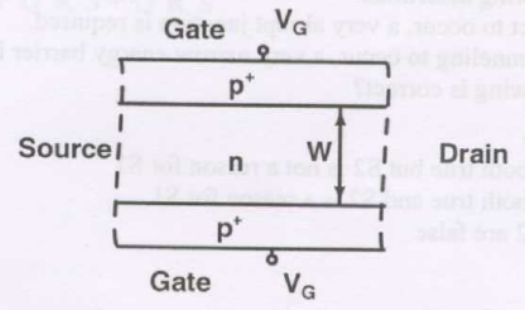
\includegraphics[width=0.6\columnwidth]{q52}
        \caption*{}
        \label{fig:q52}
    \end{figure}
    \begin{enumerate}
    \begin{multicols}{2}
        \item 4
        \item $\frac{1-\sqrt{2/V_p}}{1-\sqrt{1/\brak{2V_p}}}$
        \item $\frac{1}{2}\brak{\frac{1-\sqrt{2/V_p}}{1-\sqrt{1/\brak{2V_p}}}}$
        \item $\frac{1-\brak{2/\sqrt{V_p}}}{1-\brak{1/\brak{2\sqrt{V_p}}}}$
    \end{multicols}
    \end{enumerate}
    
    \hfill{\brak{\text{GATE EC 2008}}}

    \item Consider the Schmidt trigger circuit shown below.
    \begin{figure}[H]
        \centering
        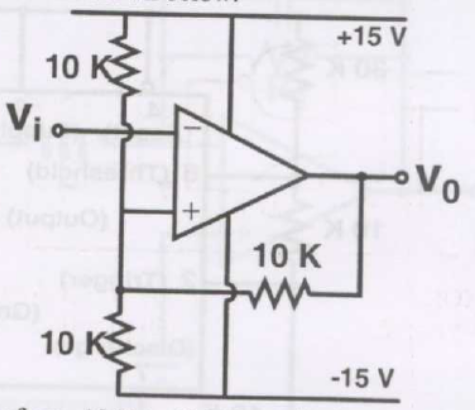
\includegraphics[width=0.4\columnwidth]{q53}
        \caption*{}
        \label{fig:q53}
    \end{figure}
    A triangular wave which goes from -12 V to 12 V is applied to the inverting input of the OPAMP. Assume that the output of the OPAMP swings from +15V to -15V. The voltage at the non-inverting input switches between
    \begin{enumerate}
        \begin{multicols}{2}
            \item -12V and +12V
            \item -7.5V and +7.5V
            \item -5V and +5V
            \item 0V and 5V
        \end{multicols}
    \end{enumerate}
    
    \hfill{\brak{\text{GATE EC 2008}}}
    
    \item The logic function implemented by the following circuit at the terminal OUT is
    \begin{figure}[H]
        \centering
        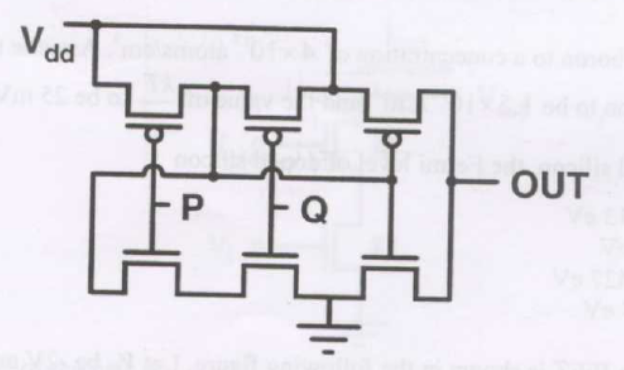
\includegraphics[width=0.4\columnwidth]{q54}
        \caption*{}
        \label{fig:q54}
    \end{figure}
    \begin{enumerate}
        \begin{multicols}{2}
            \item P NOR Q
            \item P NAND Q
            \item P OR Q
            \item P AND Q
        \end{multicols}
    \end{enumerate}

    \hfill{\brak{\text{GATE EC 2008}}}
    
    \item Consider the following assertions.\\
    S1: For Zener effect to occur, a very abrupt junction is required.\\S2: For quantum tunneling to occur, a very narrow energy barrier is required.\\Which of the following is correct?
    \begin{enumerate}
        \item Only S2 is true
        \item S1 and S2 are both true but S2 is not a reason for S1
        \item S1 and S2 are both true and S2 is a reason for S1
        \item Both S1 and S2 are false
    \end{enumerate}
    
    \hfill{\brak{\text{GATE EC 2008}}}
    
    \item The two numbers represented in signed 2's complement form are $P=11101101$ and $Q=11100110$. If Q is subtracted from P, the value obtained in signed 2's complement form is
    \begin{enumerate}
        \begin{multicols}{2}
            \item 100000111
            \item 00000111
            \item 11111001
            \item 111111001
        \end{multicols}
    \end{enumerate}

    \hfill{\brak{\text{GATE EC 2008}}}

    \item Which of the following Boolean Expressions correctly represents the relation between P, Q, R and M1?
    \begin{figure}[H]
        \centering
        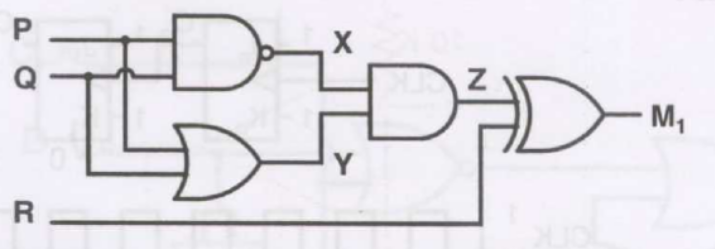
\includegraphics[width=0.7\columnwidth]{q57}
        \caption*{}
        \label{fig:q57}
    \end{figure}
    \begin{enumerate}
        \begin{multicols}{2}
            \item $M_1 = \brak{P \text{ OR } Q} \text{ XOR } R$
            \item $M_1 = \brak{P \text{ AND } Q} \text{ XOR } R$
            \item $M_1 = \brak{P \text{ NOR } Q} \text{ XOR } R$
            \item $M_1 = \brak{P \text{ XOR } Q} \text{ XOR } R$
        \end{multicols}
    \end{enumerate}
    
    \hfill{\brak{\text{GATE EC 2008}}}
    
    \item For the circuit shown in the following figure, I0-I3 are inputs to the 4:1 multiplexer. R \brak{MSB} and S are control bits.
    \begin{figure}[H]
        \centering
        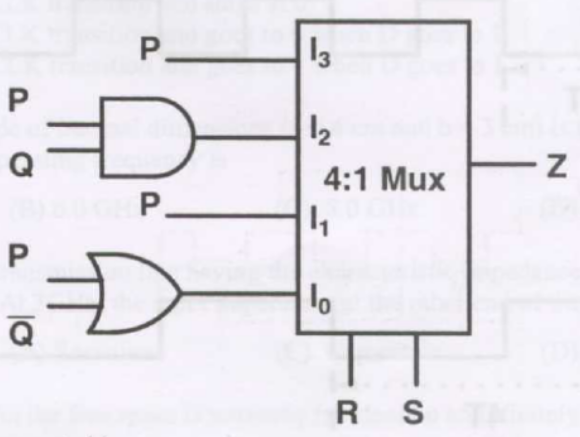
\includegraphics[width=0.6\columnwidth]{q58}
        \caption*{}
        \label{fig:q58}
    \end{figure}
    The output Z can be represented by
    \begin{enumerate}
        \item $PQ+P\overline{Q}S+\overline{Q}\overline{R}\overline{S}$
        \item $P\overline{Q}+PQ\overline{R}+\overline{P}\overline{Q}\overline{S}$
        \item $P\overline{Q}\overline{R}+\overline{P}QR+PQRS+\overline{Q}\overline{R}\overline{S}$
        \item $PQ\overline{R}+PQR\overline{S}+P\overline{Q}\overline{R}S+\overline{Q}\overline{R}\overline{S}$
    \end{enumerate}
    
    \hfill{\brak{\text{GATE EC 2008}}}
    
    \item For each of the positive edge-triggered J-K flip flop used in the following figure, the propagation delay is $\Delta T$.
    \begin{figure}[H]
        \centering
        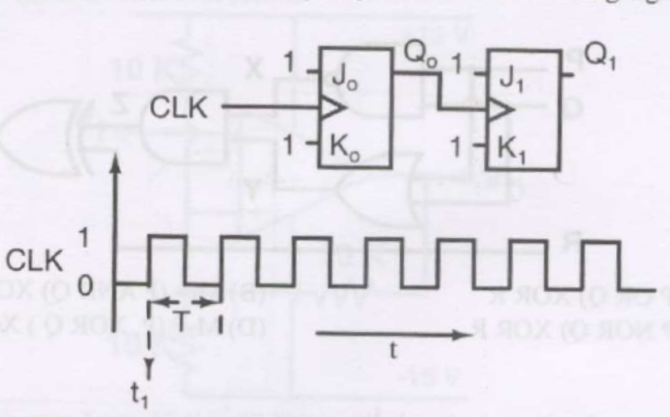
\includegraphics[width=0.8\columnwidth]{figs/q59.png}
        \caption*{}
        \label{fig:q59}
    \end{figure}
    Which of the following waveforms correctly represents the output at $Q_1$?
    \begin{figure}[H]
        \centering
        \begin{minipage}{0.45\textwidth}
            \centering
            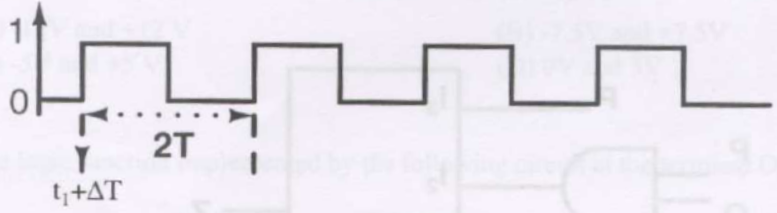
\includegraphics[width=0.9\columnwidth]{figs/q59A.png}
            \centerline{\brak{A}}
        \end{minipage}
        \hfill
        \begin{minipage}{0.45\textwidth}
            \centering
            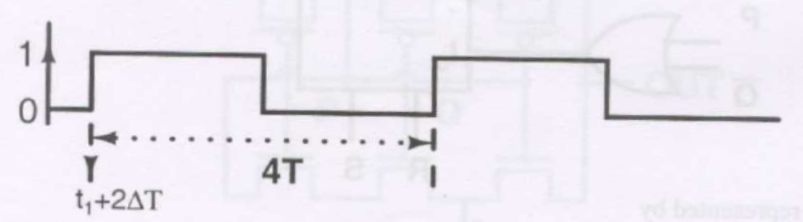
\includegraphics[width=0.9\columnwidth]{figs/q59B.png}
            \centerline{\brak{B}}
        \end{minipage}
        \vfill
        \begin{minipage}{0.45\textwidth}
            \centering
            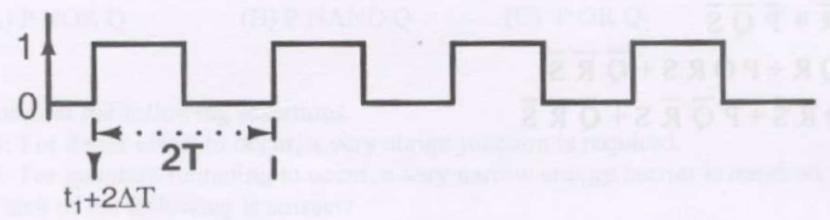
\includegraphics[width=0.9\columnwidth]{figs/q59C.png}
            \centerline{\brak{C}}
        \end{minipage}
        \hfill
        \begin{minipage}{0.45\textwidth}
            \centering
            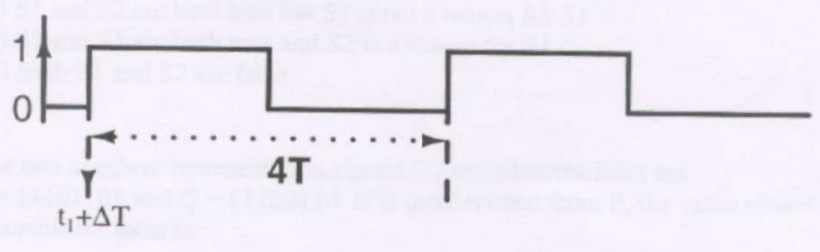
\includegraphics[width=0.9\columnwidth]{figs/q59D.png}
            \centerline{\brak{D}}
        \end{minipage}
        \caption*{}
        \label{fig:q59_options}
    \end{figure}

    \hfill{\brak{\text{GATE EC 2008}}}
    
    \item For the circuit shown in the figure, D has a transition from 0 to 1 after CLK changes from 1 to 0. Assume gate delays to be negligible.
    \begin{figure}[H]
        \centering
        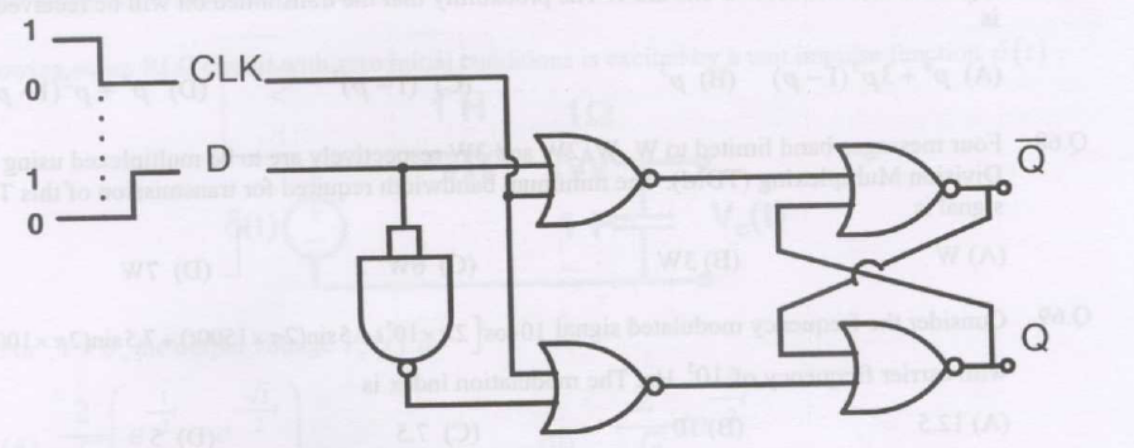
\includegraphics[width=0.8\columnwidth]{q60}
        \caption*{}
        \label{fig:q60}
    \end{figure}
    Which of the following statements is true?
    \begin{enumerate}
        \item Q goes to 1 at the CLK transition and stays at 1.
        \item Q goes to 0 at the CLK transition and stays at 0.
        \item Q goes to 1 at the CLK transition and goes to 0 when D goes to 1.
        \item Q goes to 0 at the CLK transition and goes to 1 when D goes to 1.
    \end{enumerate}
    
    \hfill{\brak{\text{GATE EC 2008}}}
    
    \item A rectangular waveguide of internal dimensions \brak{$a=4$ cm and $b=3$ cm} is to be operated in $TE_{11}$ mode. The minimum operating frequency is
    \begin{enumerate}
        \begin{multicols}{2}
            \item 6.25 GHz
            \item 6.0 GHz
            \item 5.0 GHz
            \item 3.75 GHz
        \end{multicols}
    \end{enumerate}
    
    \hfill{\brak{\text{GATE EC 2008}}}
    
    \item One end of a loss-less transmission line having the characteristic impedance of 75$\ohm$ and length of 1cm is short-circuited. At 3GHz, the input impedance at the other end of the transmission line is
    \begin{enumerate}
        \begin{multicols}{2}
            \item 0
            \item Resistive
            \item Capacitive
            \item Inductive
        \end{multicols}
    \end{enumerate}
    
    \hfill{\brak{\text{GATE EC 2008}}}
    
    \item A uniform plane wave in the free space is normally incident on an infinitely thick dielectric slab \brak{dielectric constant $\epsilon_r=9$}. The magnitude of the reflection coefficient is
    \begin{enumerate}
        \begin{multicols}{4}
            \item 0
            \item 0.3
            \item 0.5
            \item 0.8
        \end{multicols}
    \end{enumerate}
    
    \hfill{\brak{\text{GATE EC 2008}}}
    
    \item In the design of a single mode step index optical fiber close to upper cut-off, the single-mode operation is NOT preserved if
    \begin{enumerate}
        \item radius as well as operating wavelength are halved
        \item radius as well as operating wavelength are doubled
        \item radius is halved and operating wavelength is doubled
        \item radius is doubled and operating wavelength is halved
    \end{enumerate}
    
    \hfill{\brak{\text{GATE EC 2008}}}

    \item At 20 GHz, the gain of a parabolic dish antenna of 1 meter diameter and 70\% efficiency is
    \begin{enumerate}
        \begin{multicols}{4}
            \item 15 dB
            \item 25 dB
            \item 35 dB
            \item 45 dB
        \end{multicols}
    \end{enumerate}
    
    \hfill{\brak{\text{GATE EC 2008}}}
    
    \item Noise with double-sided power spectral density of K over all frequencies is passed through a RC low pass filter with 3 dB cut-off frequency of $f_c$. The noise power at the filter output is
    \begin{enumerate}
        \begin{multicols}{2}
            \item K
            \item $K f_c$
            \item $K \pi f_c$
            \item $\infty$
        \end{multicols}
    \end{enumerate}
    
    \hfill{\brak{\text{GATE EC 2008}}}

    \item Consider a Binary Symmetric Channel \brak{BSC} with probability of error being p. To transmit a bit, say 1, we transmit a sequence of three 1s. The receiver will interpret the received sequence to represent 1 if at least two bits are 1. The probability that the transmitted bit will be received in error is
    \begin{enumerate}
    \begin{multicols}{4}
        \item $p^3+3p^2\brak{1-p}$
        \item $p^3$
        \item $\brak{1-p}^3$
        \item $p^3+p^2\brak{1-p}$
    \end{multicols}
    \end{enumerate}
    
    \hfill{\brak{\text{GATE EC 2008}}}
    
    \item Four messages band limited to W, W, 2W and 3W respectively are to be multiplexed using Time Division Multiplexing \brak{TDM}. The minimum bandwidth required for transmission of this TDM signal is
    \begin{enumerate}
        \begin{multicols}{4}
            \item W
            \item 3W
            \item 6W
            \item 7W
        \end{multicols}
    \end{enumerate}
    
    \hfill{\brak{\text{GATE EC 2008}}}
    
    \item Consider the frequency modulated signal $10\cos[2\pi \times 10^5 t + 5\sin\brak{2\pi \times 1500t} + 7.5\sin\brak{2\pi \times 1000t}]$ with carrier frequency of $10^5$ Hz. The modulation index is
    \begin{enumerate}
        \begin{multicols}{4}
            \item 12.5
            \item 10
            \item 7.5
            \item 5
        \end{multicols}
    \end{enumerate}
    
    \hfill{\brak{\text{GATE EC 2008}}}
    
    \item The signal $\cos\omega_c t + 0.5 \cos\omega_m t \sin\omega_c t$ is
    \begin{enumerate}
        \begin{multicols}{2}
            \item FM only
            \item AM only
            \item both AM and FM
            \item neither AM nor FM
        \end{multicols}
    \end{enumerate}

    \hfill{\brak{\text{GATE EC 2008}}}
    
    \item A speech signal, band limited to 4 kHz and peak voltage varying between +5V and -5V, is sampled at the Nyquist rate. Each sample is quantized and represented by 8 bits.
    
    If the bits 0 and 1 are transmitted using bipolar pulses, the minimum bandwidth required for distortion free transmission is
    \begin{enumerate}
        \begin{multicols}{4}
            \item 64 kHz
            \item 32 kHz
            \item 8 kHz
            \item 4 kHz
        \end{multicols}
    \end{enumerate}
    
    \hfill{\brak{\text{GATE EC 2008}}}

    \item Assuming the signal to be uniformly distributed between its peak to peak value, the signal to noise ratio at the quantizer output is
    \begin{enumerate}
        \begin{multicols}{4}
            \item 16 dB
            \item 32 dB
            \item 48 dB
            \item 64 dB
        \end{multicols}
    \end{enumerate}
    
    \hfill{\brak{\text{GATE EC 2008}}}

    \item The number of quantization levels required to reduce the quantization noise by a factor of 4 would be
    \begin{enumerate}
        \begin{multicols}{4}
            \item 1024
            \item 512
            \item 256
            \item 64
        \end{multicols}
    \end{enumerate}
    
    \hfill{\brak{\text{GATE EC 2008}}}

    The following series RLC circuit with zero initial conditions is excited by a unit impulse function $\delta\brak{t}$.
    \begin{figure}[H]
        \centering
        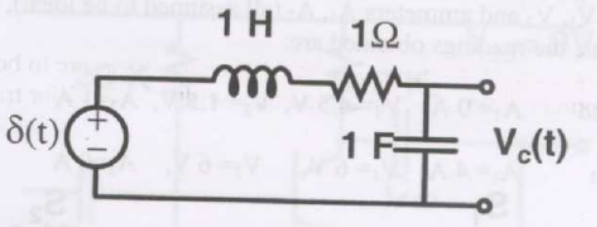
\includegraphics[width=0.5\columnwidth]{figs/q74.png}
        \caption*{}
        \label{fig:q74}
    \end{figure}
    \item For $t>0$, the output voltage $V_c\brak{t}$ is
    \begin{enumerate}
    \begin{multicols}{2}
        \item $\frac{2}{\sqrt{3}}\brak{e^{-\frac{1}{2}t}-e^{\frac{\sqrt{3}}{2}t}}$
        \item $\frac{2}{\sqrt{3}}te^{-\frac{1}{2}t}$
        \item $\frac{2}{\sqrt{3}}e^{-\frac{1}{2}t}\cos\brak{\frac{\sqrt{3}}{2}t}$
        \item $\frac{2}{\sqrt{3}}e^{-\frac{1}{2}t}\sin\brak{\frac{\sqrt{3}}{2}t}$
    \end{multicols}
    \end{enumerate}
    
    \hfill{\brak{\text{GATE EC 2008}}}
    
    \item For $t>0$, the voltage across the resistor is
    \begin{enumerate}
    \begin{multicols}{2}
        \item $\frac{1}{\sqrt{3}}\brak{e^{-\frac{\sqrt{3}}{2}t}-e^{-\frac{1}{2}t}}$
        \item $e^{-\frac{1}{2}t}[\cos\brak{\frac{\sqrt{3}t}{2}}-\frac{1}{\sqrt{3}}\sin\brak{\frac{\sqrt{3}t}{2}}]$
        \item $\frac{2}{\sqrt{3}}e^{-\frac{1}{2}t}\sin\brak{\frac{\sqrt{3}t}{2}}$
        \item $\frac{2}{\sqrt{3}}e^{-\frac{1}{2}t}\cos\brak{\frac{\sqrt{3}t}{2}}$
    \end{multicols}
    \end{enumerate}
    
    \hfill{\brak{\text{GATE EC 2008}}}

    \item[] A two-port network shown below is excited by external dc sources. The voltages and the currents are measured with voltmeters $V_1, V_2$ and ammeters $A_1, A_2$ \brak{all assumed to be ideal}, as indicated. Under following switch conditions, the readings obtained are:
    \begin{enumerate}[label=\roman*.]
        \item $S_1$-Open, $S_2$-Closed $A_1=0A, V_1=4.5V, V_2=1.5V, A_2=1A$
        \item $S_1$-Closed, $S_2$-Open $A_1=4A, V_1=6V, V_2=6V, A_2=0A$
    \end{enumerate}
    
    \begin{figure}[H]
        \centering
        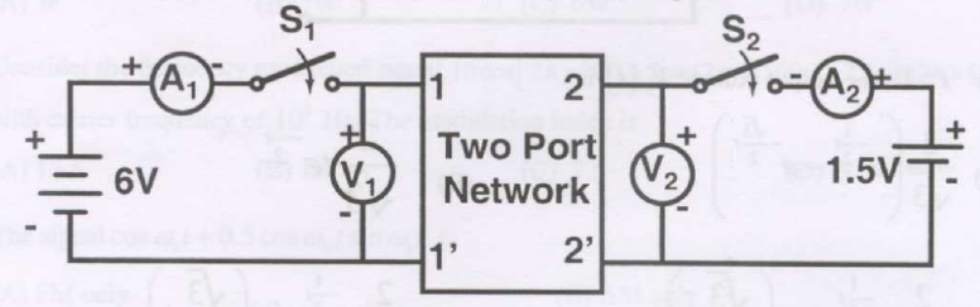
\includegraphics[width=0.8\columnwidth]{figs/q76.png}
        \caption*{}
        \label{fig:q76}
    \end{figure}
    
    \item The z-parameter matrix for this network is
    \begin{enumerate}
        \begin{multicols}{2}
            \item $\myvec{1.5 & 1.5 \\ 4.5 & 1.5}$
            \item $\myvec{1.5 & 4.5 \\ 1.5 & 4.5}$
            \item $\myvec{1.5 & 4.5 \\ 1.5 & 1.5}$
            \item $\myvec{4.5 & 1.5 \\ 1.5 & 4.5}$
        \end{multicols}
    \end{enumerate}
    
    \hfill{\brak{\text{GATE EC 2008}}}
    
    \item The h-parameter matrix for this network is
    \begin{enumerate}
        \begin{multicols}{2}
            \item $\myvec{-3 & 3 \\ -1 & 0.67}$
            \item $\myvec{-3 & -1 \\ 3 & 0.67}$
            \item $\myvec{3 & 3 \\ 1 & 0.67}$
            \item $\myvec{3 & 1 \\ -3 & -0.67}$
        \end{multicols}
    \end{enumerate}
    
    \hfill{\brak{\text{GATE EC 2008}}}
    
    \item[] In the following network, the switch is closed at $t=0-$ and the sampling starts from $t=0$. The sampling frequency is 10 Hz.
    \begin{figure}[H]
        \centering
        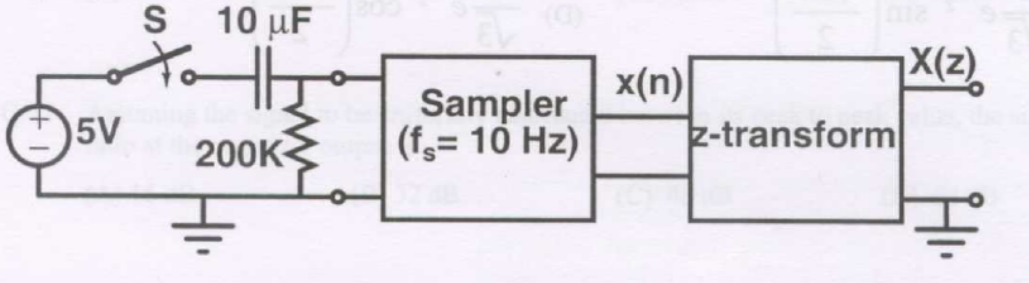
\includegraphics[width=\columnwidth]{q78}
        \caption*{}
        \label{fig:q78}
    \end{figure}
    
    \item The samples $x\brak{n}$ \brak{n=0,1,2,...} are given by
    \begin{enumerate}
        \begin{multicols}{2}
            \item $5\brak{1-e^{-0.05n}}$
            \item $5e^{-0.05n}$
            \item $5\brak{1-e^{-5n}}$
            \item $5e^{-5n}$
        \end{multicols}
    \end{enumerate}
    
    \hfill{\brak{\text{GATE EC 2008}}}
    
    \item The expression and the region of convergence of the z-transform of the sampled signal are
    \begin{enumerate}
        \begin{multicols}{2}
            \item $\frac{5z}{z-e^{-5}}, |z|<e^{-5}$
            \item $\frac{5z}{z-e^{-0.05}}, |z|<e^{-0.05}$
            \item $\frac{5z}{z-e^{-0.05}}, |z|>e^{-0.05}$
            \item $\frac{5z}{z-e^{-5}}, |z|>e^{-5}$
        \end{multicols}
    \end{enumerate}

    \hfill{\brak{\text{GATE EC 2008}}}
    
    \item[] In the following transistor circuit, $V_{BE} = 0.7V, r_e = 25mV/I_E$, and $\beta$ and all the capacitances are very large.
    \begin{figure}[H]
        \centering
        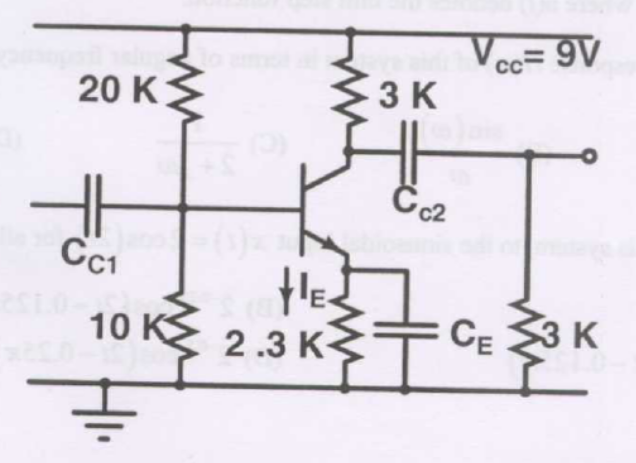
\includegraphics[width=0.6\columnwidth]{q80}
        \caption*{}
        \label{fig:q80}
    \end{figure}
    
    \item The value of DC current $I_E$ is
    \begin{enumerate}
        \begin{multicols}{4}
            \item 1 mA
            \item 2 mA
            \item 5 mA
            \item 10 mA
        \end{multicols}
    \end{enumerate}

    \hfill{\brak{\text{GATE EC 2008}}}
    
    \item The mid-band voltage gain of the amplifier is approximately
    \begin{enumerate}
        \begin{multicols}{4}
            \item -180
            \item -120
            \item -90
            \item -60
        \end{multicols}
    \end{enumerate}

    \hfill{\brak{\text{GATE EC 2008}}}
    
    \item[] In the following circuit, the comparator output is logic "1" if $V_1 > V_2$ and is logic "0" otherwise. The D/A conversion is done as per the relation $V_{DAC} = \sum_{n=0}^{3} 2^{n-1}b_n$ Volts, where $b_3$ \brak{MSB}, $b_2, b_1$ and $b_0$ \brak{LSB} are the counter outputs. The counter starts from the clear state.
    \begin{figure}[H]
        \centering
        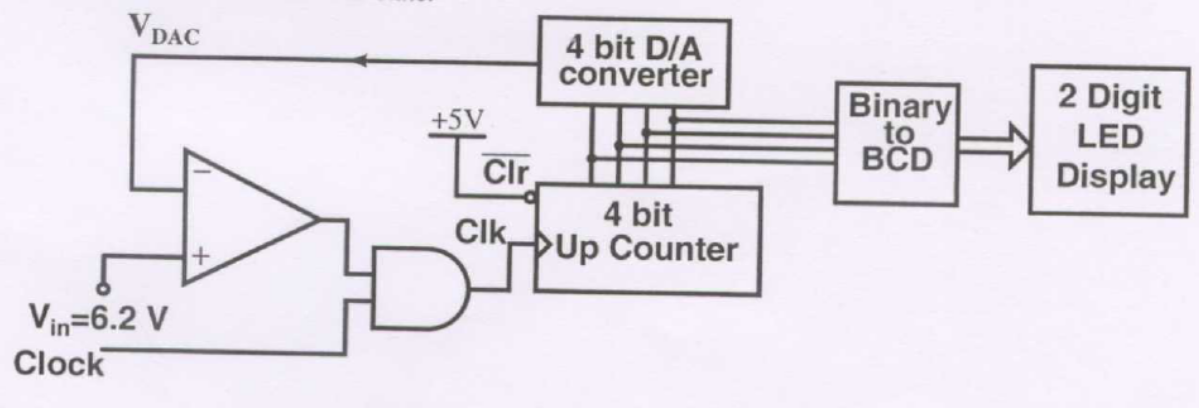
\includegraphics[width=\columnwidth]{q82}
        \caption*{}
        \label{fig:q82}
    \end{figure}
    
    \item The stable reading of the LED displays is
    \begin{enumerate}
        \begin{multicols}{4}
            \item 06
            \item 07
            \item 12
            \item 13
        \end{multicols}
    \end{enumerate}
    
    \hfill{\brak{\text{GATE EC 2008}}}
    
    \item The magnitude of the error between $V_{DAC}$ and $V_{in}$ at steady state in volts is
    \begin{enumerate}
        \begin{multicols}{4}
            \item 0.2
            \item 0.3
            \item 0.5
            \item 1.0
        \end{multicols}
    \end{enumerate}
    
    \hfill{\brak{\text{GATE EC 2008}}}
    
    \item[] The impulse response $h\brak{t}$ of a linear time-invariant continuous time system is given by $h\brak{t}=\exp\brak{-2t}u\brak{t}$, where $u\brak{t}$ denotes the unit step function.
    
    \item The frequency response $H\brak{\omega}$ of this system in terms of angular frequency $\omega$, is given by $H\brak{\omega}=$
    \begin{enumerate}
        \begin{multicols}{4}
            \item $\frac{1}{1+j2\omega}$
            \item $\frac{\sin\brak{\omega}}{\omega}$
            \item $\frac{1}{2+j\omega}$
            \item $\frac{j\omega}{2+j\omega}$
        \end{multicols}
    \end{enumerate}
    
    \hfill{\brak{\text{GATE EC 2008}}}
    
    \item The output of this system, to the sinusoidal input $x\brak{t} = 2\cos\brak{2t}$ for all time t, is
    \begin{enumerate}
        \begin{multicols}{2}
            \item 0
            \item $2^{-0.25}\cos\brak{2t-0.125\pi}$
            \item $2^{-0.5}\cos\brak{2t-0.125\pi}$
            \item $2^{-0.5}\cos\brak{2t-0.25\pi}$
        \end{multicols}
    \end{enumerate}
    
    \hfill{\brak{\text{GATE EC 2008}}}

\end{enumerate}
\end{document}

